\documentclass[xcolor=svgnames]{beamer}
\usepackage[utf8]{inputenc}
\usepackage[english]{babel}

\usetheme{Proso}

\title[Student Modeling]{Student Modeling in Online Educational Systems}
\author{Jan Papoušek}
\institute{Masaryk University Brno}
\date{\today}

\begin{document}
% --------------------------- SLIDE --------------------------------------------
\frame[plain]{\titlepage}
% ------------------------------------------------------------------------------
% --------------------------- SLIDE --------------------------------------------
\begin{frame}
	\frametitle{Platforms for Online Education}

	\begin{columns}[2]
		\column{.5\textwidth}
		\begin{center}
			
\includegraphics[width=0.95\textwidth]{2013-VV041-student-modeling/coursera.jpg}

			
\includegraphics[width=.7\textwidth]{2013-VV041-student-modeling/khanacademy.png}
		\end{center}
		\column{.5\textwidth}
		\begin{center}
			
\includegraphics[width=.5\textwidth]{2013-VV041-student-modeling/udacity.png}

			
\includegraphics[width=0.7\textwidth]{2013-VV041-student-modeling/edx.jpg}
		\end{center}
	\end{columns}
\end{frame}
% ------------------------------------------------------------------------------
% --------------------------- SLIDE --------------------------------------------
\begin{frame}
	\frametitle{Platforms for Online Education}
	\begin{center}
		\Huge millions of students
	\end{center}

	\bigskip
	\hrule

	\medskip
	\begin{itemize}
		\item 	high accessibility
		\item 	huge volume of \textit{passive} content -- videos, slides, e-books, \ldots
		\item 	\alert{it is necessary to practice}
						\begin{itemize}
							\item 	adaptive systems for practicing
						\end{itemize}
	\end{itemize}
\end{frame}
% ------------------------------------------------------------------------------
% --------------------------- SLIDE --------------------------------------------
\begin{frame}
	\frametitle{Systems for Practicing}

	\begin{columns}[T]
		\column{.5\textwidth}
		\textbf{Student}
		\begin{itemize}
			\item 	tries to solve the exercises
		\end{itemize}

		\bigskip
		\bigskip

		\begin{itemize}
			\item 	Which exercies should be chosen for practicing?
			\item 	student's skill / knowledge -- How does it look like?
		\end{itemize}

		\column{.5\textwidth}
		\textbf{Expert / Teacher}
		\begin{itemize}
			\item 	the author of exercises
		\end{itemize}

		\bigskip
		\bigskip
		\begin{itemize}
			\item 	What's the progress of students?
			\item 	parameters of exercises -- How do the look like?
		\end{itemize}
	\end{columns}

\end{frame}
% ------------------------------------------------------------------------------
% --------------------------- SLIDE --------------------------------------------
\begin{frame}
	\frametitle{Types of Exercises}

	\begin{center}
		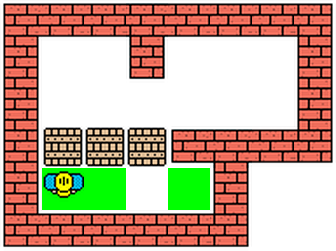
\includegraphics[width=.6\textwidth]{2013-VV041-student-modeling/sokoban.png}
	\end{center}
\end{frame}
% ------------------------------------------------------------------------------
% --------------------------- SLIDE --------------------------------------------
\begin{frame}
	\frametitle{Types of Exercises}
	\transduration{1}
	How many blue points do you see? Remaining seconds: {\Huge\only<1>{10}\only<2>{9}\only<3>{8}\only<4>{7}\only<5>{6}\only<6>{5}\only<7>{4}\only<8>{3}\only<9>{2}\only<10>{1}}

	\begin{center}
		\medskip
		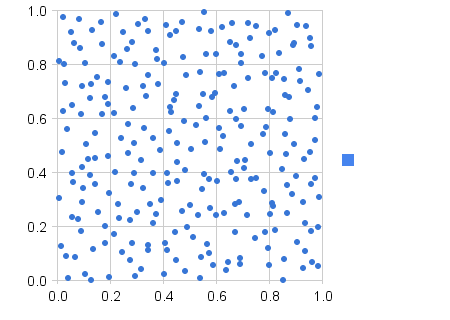
\includegraphics[width=.7\textwidth]{2013-VV041-student-modeling/random-plot.png}
	\end{center}
\end{frame}
% ------------------------------------------------------------------------------
% --------------------------- SLIDE --------------------------------------------
\begin{frame}
\end{frame}
% ------------------------------------------------------------------------------
% --------------------------- SLIDE --------------------------------------------
\begin{frame}
	\frametitle{Types of Exercises}
	What is the name of the state highlighted on the map?
	\begin{itemize}
		\item 	Turkey or Egypt?
	\end{itemize}
	\begin{center}
		\medskip
		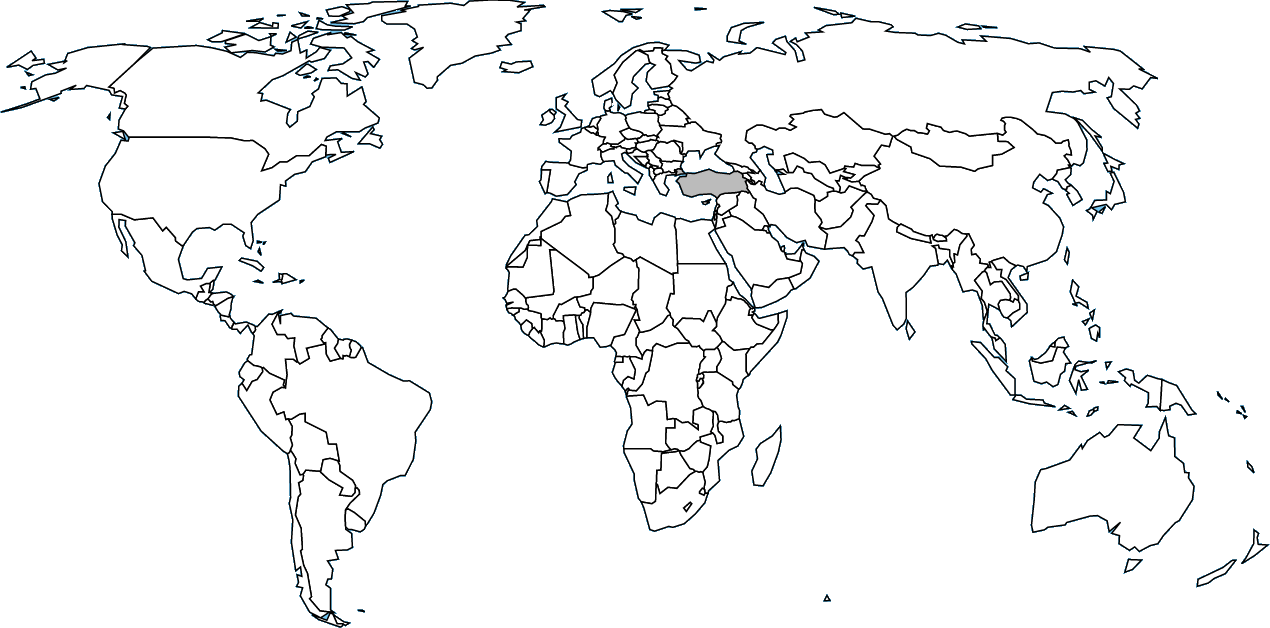
\includegraphics[width=.95\textwidth]{2013-VV041-student-modeling/map.png}
	\end{center}
\end{frame}
% ------------------------------------------------------------------------------
% --------------------------- SLIDE --------------------------------------------
\begin{frame}
	\frametitle{Types of Exercises}
	Compute the determinant of the following matrix:
	\begin{center}
	\Huge
$$
\begin{pmatrix}
	\cos x & - \sin x \\
	\sin x & \cos x
\end{pmatrix}
$$
	\end{center}
\end{frame}
% ------------------------------------------------------------------------------
% --------------------------- SLIDE --------------------------------------------
\begin{frame}
	\frametitle{Types of Exercises}

	\begin{itemize}
		\item 	\textbf{by result}
			\begin{itemize}
				\item time
				\item correctness: yes / no
				\item correctness: percentage
			\end{itemize}
		\item 	\textbf{by possible learning}
			\begin{itemize}
				\item no learning
				\item some learning possible
			\end{itemize}
	\end{itemize}
\end{frame}
% ------------------------------------------------------------------------------
% --------------------------- SLIDE --------------------------------------------
\begin{frame}
	\frametitle{Model I -- Time}

	\bigskip
	solution times are lognormal distributed -- logarithm of time is used

	\bigskip
	\begin{columns}
		\column{.45\textwidth}
		\textbf{student}
		\begin{description}
			\item[$\Theta$]	skill
		\end{description}
		\textbf{exercise}
		\begin{description}
			\item[$a_i$] discrimination
			\item[$b_i$] difficulty
			\item[$c_i$] pseudo-guessing
		\end{description}
		\column{.55\textwidth}
		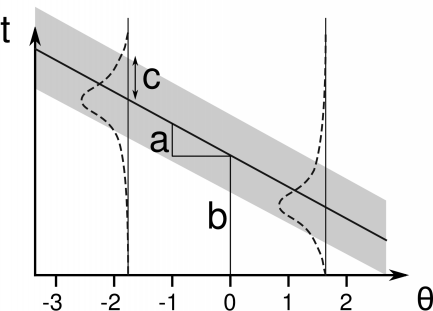
\includegraphics[width=\textwidth]{2013-VV041-student-modeling/time-model.png}
	\end{columns}
	\begin{center}
		$$
		t_i(\Theta) = b_i + a_i\Theta + \mathcal{N}(0, c_i)
		$$
	\end{center}
\end{frame}
% ------------------------------------------------------------------------------
% --------------------------- SLIDE --------------------------------------------
\begin{frame}
	\frametitle{Model I -- Time}

	\begin{center}
		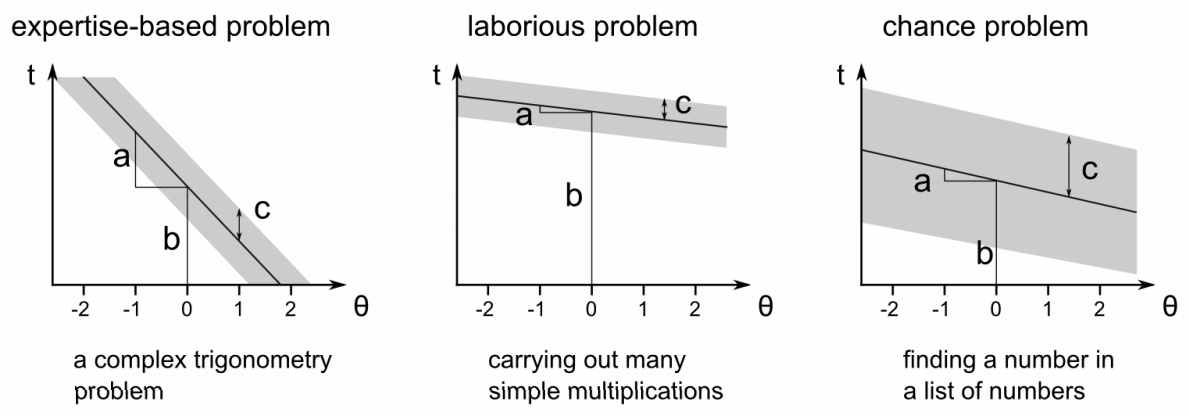
\includegraphics[width=.95\textwidth]{2013-VV041-student-modeling/time-model-types.png}
	\end{center}
\end{frame}
% ------------------------------------------------------------------------------
% --------------------------- SLIDE --------------------------------------------
\begin{frame}
	\frametitle{Model I -- Time}

	\begin{center}
		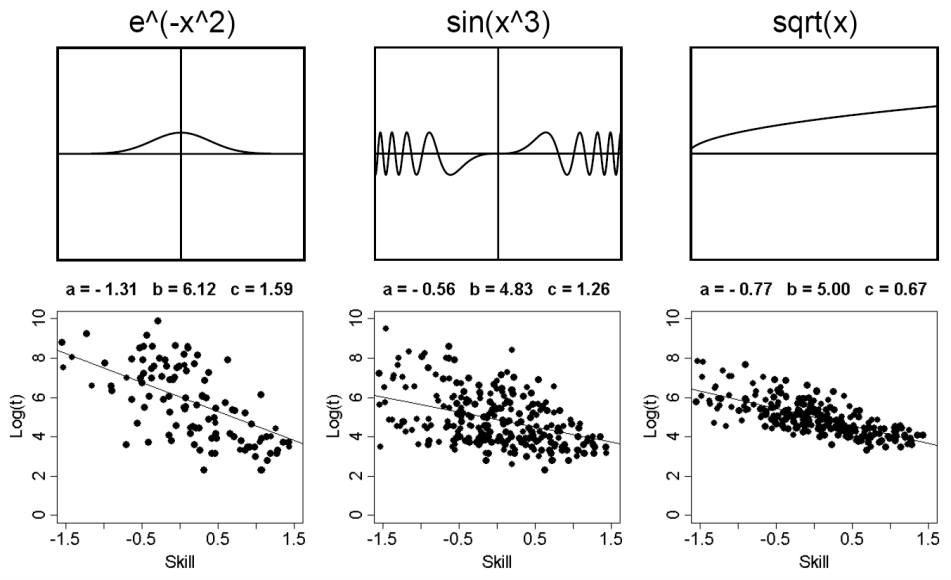
\includegraphics[width=.95\textwidth]{2013-VV041-student-modeling/time-model-examples.png}
	\end{center}
\end{frame}
% ------------------------------------------------------------------------------
% --------------------------- SLIDE --------------------------------------------
\begin{frame}
	\frametitle{Model II -- Correctness}
	\begin{columns}
		\column{.45\textwidth}
		\textbf{student}
		\begin{description}
			\item[$\Theta$]	skill
		\end{description}
		\textbf{exercise}
		\begin{description}
			\item[$a_i$] discrimination
			\item[$b_i$] difficulty
			\item[$c_i$] pseudo-guessing
		\end{description}
		\column{.55\textwidth}
		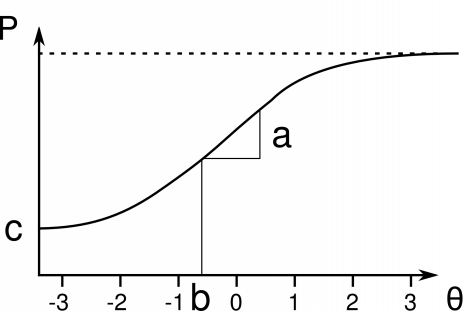
\includegraphics[width=\textwidth]{2013-VV041-student-modeling/correctness-model.png}
	\end{columns}
	\begin{center}
		$$
		P_i(\Theta) = c_i + \frac{1 - c_i}{1 + e^{-a_i(\Theta - b_i)}}
		$$
	\end{center}
\end{frame}
% ------------------------------------------------------------------------------
% --------------------------- SLIDE --------------------------------------------
\begin{frame}
	\frametitle{Model II -- Correctness}

	\begin{center}
		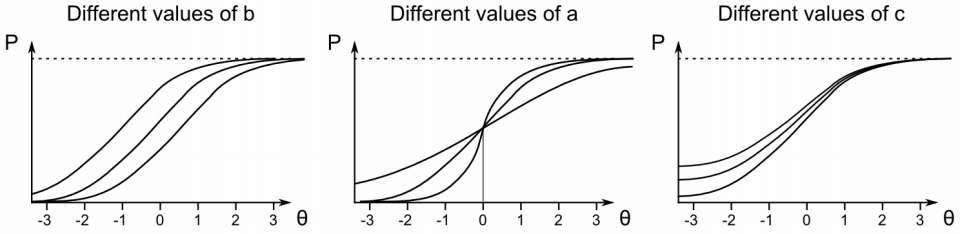
\includegraphics[width=.95\textwidth]{2013-VV041-student-modeling/correctness-model-types.png}
	\end{center}
\end{frame}
% ------------------------------------------------------------------------------
% --------------------------- SLIDE --------------------------------------------
\begin{frame}
	\frametitle{Model I vs. Model II}

	\begin{center}
		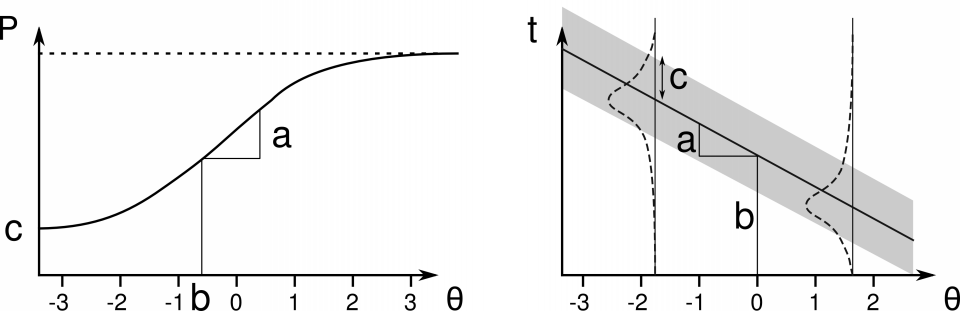
\includegraphics[width=.95\textwidth]{2013-VV041-student-modeling/models-compare.png}
	\end{center}
\end{frame}
% ------------------------------------------------------------------------------
% --------------------------- SLIDE --------------------------------------------
\begin{frame}
	\frametitle{Conclusion}
	\begin{itemize}
		\item 	models are used to improve the behaviour of systems for practicing
			\begin{itemize}
				\item 	prediction
				\item 	feedback
			\end{itemize}
		\item 	different types of exercises \\
						$\Rightarrow$ different parameters \\
						$\Rightarrow$ different models
	\end{itemize}
\end{frame}
% ------------------------------------------------------------------------------
% --------------------------- SLIDE --------------------------------------------
\begin{frame}
	\begin{center}
		{\Huge QUESTIONS?}
	\end{center}
\end{frame}
% ------------------------------------------------------------------------------
% --------------------------- SLIDE --------------------------------------------
\begin{frame}[allowframebreaks]
	\frametitle<presentation>{Bibliography}
	\bibliographystyle{plain}
	\nocite{Jarusek2013thesis}
	\bibliography{bibliography}
\end{frame}
% ------------------------------------------------------------------------------
\end{document}
